\documentclass[10pt]{article}
\usepackage[margin=0.7in]{geometry}
\usepackage[T1]{fontenc}
\usepackage{lmodern,graphicx,booktabs,hyperref}
\hypersetup{colorlinks=true,urlcolor=blue}
\setlength{\parindent}{0pt}\setlength{\parskip}{6pt}\setlength{\emergencystretch}{3em}
\begin{document}
{\Large\bfseries CPU source reconciliation and matched-comparison preparation}

23 November 2026. Producer observations, PCC unverified.
Unsigned source/software record: \texttt{PCC-20261123-9c9ba9}.

Both source-separated variants build with original Rust 1.99.1 and each passes
47 library checks, zero failed/ignored; two other worker harnesses are empty.
Seven copied driver tests and strict all-target Clippy pass; the separate audit
test harness is empty. These are qualification results, before new solver data.

\begin{center}\begin{tabular}{lll}\toprule
Variant & Exact library origin & Qualified input set\\\midrule
Staged numerator parent & \texttt{4939261c9fcc} &108 files\\
Reverse-pass candidate & \texttt{c47886258a0e}, current &108 files\\\bottomrule
\end{tabular}\end{center}
The sole source difference is \texttt{crates/hashed-ecdl-cpu/src/lib.rs}.
It removes one numerator vector and reschedules numerator derivation into the
reverse pass. Curve formulas, denominators, witness order and replay remain.
Total loads, machine work and peak memory have not been measured by this check.

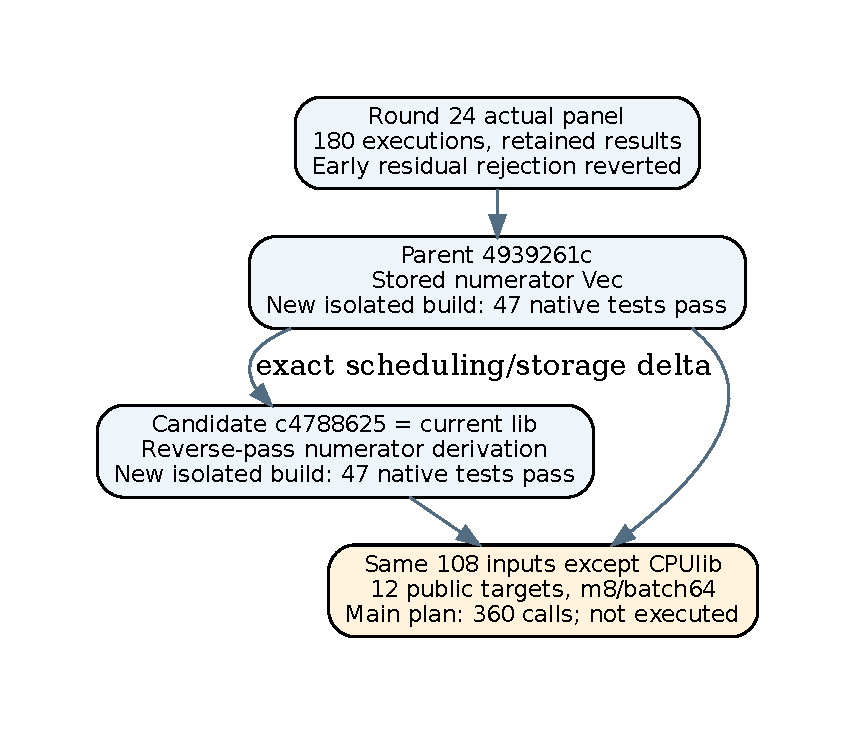
\includegraphics[width=\linewidth,height=3.1in,keepaspectratio]{source-map.pdf}

\textbf{Historical correction.} Round24's preparation README is stale. Actual
EXECUTION/rows/summary records exist: 180 calls, 162 measured, 18 warmups. They led to
reverting early residual rejection at the inspected L0 scope. The prior scale
README/journal combined absence statement about 24/25 was wrong for 24; sibling
errata correct it without changing frozen evidence. Source review10 independently
reconciles 180 rows/108 summary entries and the exact historical/current lib files.
The original native-baseline README's statement that reconciliation was needed
remains true. Round25 has 31 preparation files and no result tree at \texttt{310d7fb0}.

\textbf{Prospective local design.} Unchanged scale workers, six fixed curves,
two public targets per curve, m8/batch64. Logical a/c use one copied parent binary;
b uses the candidate. Native argv remains u in exclusive output directories.
Collector IDs include case+seed and round; native replicate/warmup fields remain.
Planned main census: 360 calls, 36 warmups/324 measured; no main data yet.

\textbf{Preflight before main freeze.} One warmup-only 36-cell round, 300s ceiling,
120s worker/60s external replay, one attempt/no retries, 4GiB worker virtual limit,
existing 15,032,385,536-byte whole-cgroup guard. Complete certificates/counters
must agree; every cell has Native replay and OpenSSL point/binding/corruption
checks. Fixed affinity is not host isolation. L0 clocks are descriptive only.
Require preflight runtime plus 25\% margin to fit the 1800s proposed main ceiling.

\textbf{Evidence and scope.} Main protocol is not yet frozen. The original
24-call 40-bit cohort, round25 cloud protocol/attempt and 84-case tensor obligations
remain unchanged. Local only; no S3 or added cloud spend. Source/status review
and archive hashes do not supply authenticated independent execution, a novel
mechanism, total-operation price or ranked timing. KB tools unavailable; exact
repository sources supply the scoped prior-work review.

\small Study: \path{research/hashed_ecdl_cpu_compare_20261123}.\par
\url{https://github.com/isogeny-labs/crypto/pull/4996}
\end{document}
